\section{Σχεδιασμός του Κύκλου}
\subsection{Σχεδιασμός Κύκλου μέσω της αλγεβρικής εξίσωσης}

Έστω κύκλος με κέντρο $K(x_c, y_c)$ και ακτίνα $r$. Τότε η αλγεβρική του εξίσωση είναι:
\begin{equation}
	(x-x_c)^2 + (y-y_c)^2 = r^2
	\label{eq:1}
\end{equation}

Λύνωντας την $\eqref{eq:1}$ ως προς $y$ προκύπτει:
\[
	y = f(x) = y_c \pm \sqrt{r^2- (x-x_c)^2}
\]

Είναι προφανές, ότι απαιτούνται πολλοί υπολογισμοί σε κάθε βήμα. Σαν να μην έφτανε αυτό, απαιτείται και υπολογισμός της τετραγωνικής ρίζας, που "βαραίνει" ακόμα περισσότερο τους υπολογισμούς μας.

Αυτό έχει ως αποτέλεσμα, να μην είναι ομοιόμορφη η κατανομή των φωτιζόμενων pixelσ και ειδικά στο κομμμάτι μεταξύ $45^\circ$ και $90^\circ$.

\begin{lstlisting}[caption={Αλγόριθμος Σχεδιασμού κύκλου μέσω αλγεβρικής εξίσωσης}]
function circlePlot(xc, yc, r)
	# (xc, yc) are the coordinates of the circle's centre
	# r is the radius of the circle
	x = xc-r 
    i = 1
	while x <= xc+r
        y1 = yc + sqrt( r^2-(x-xc)^2 )
        plot(x,y1)
        y2 = yc - sqrt( r^2-(x-xc)^2 )
        plot(x,y2)
        x = x + 1 
	end
end
\end{lstlisting}


\begin{figure}[hbt]
  \begin{center}
	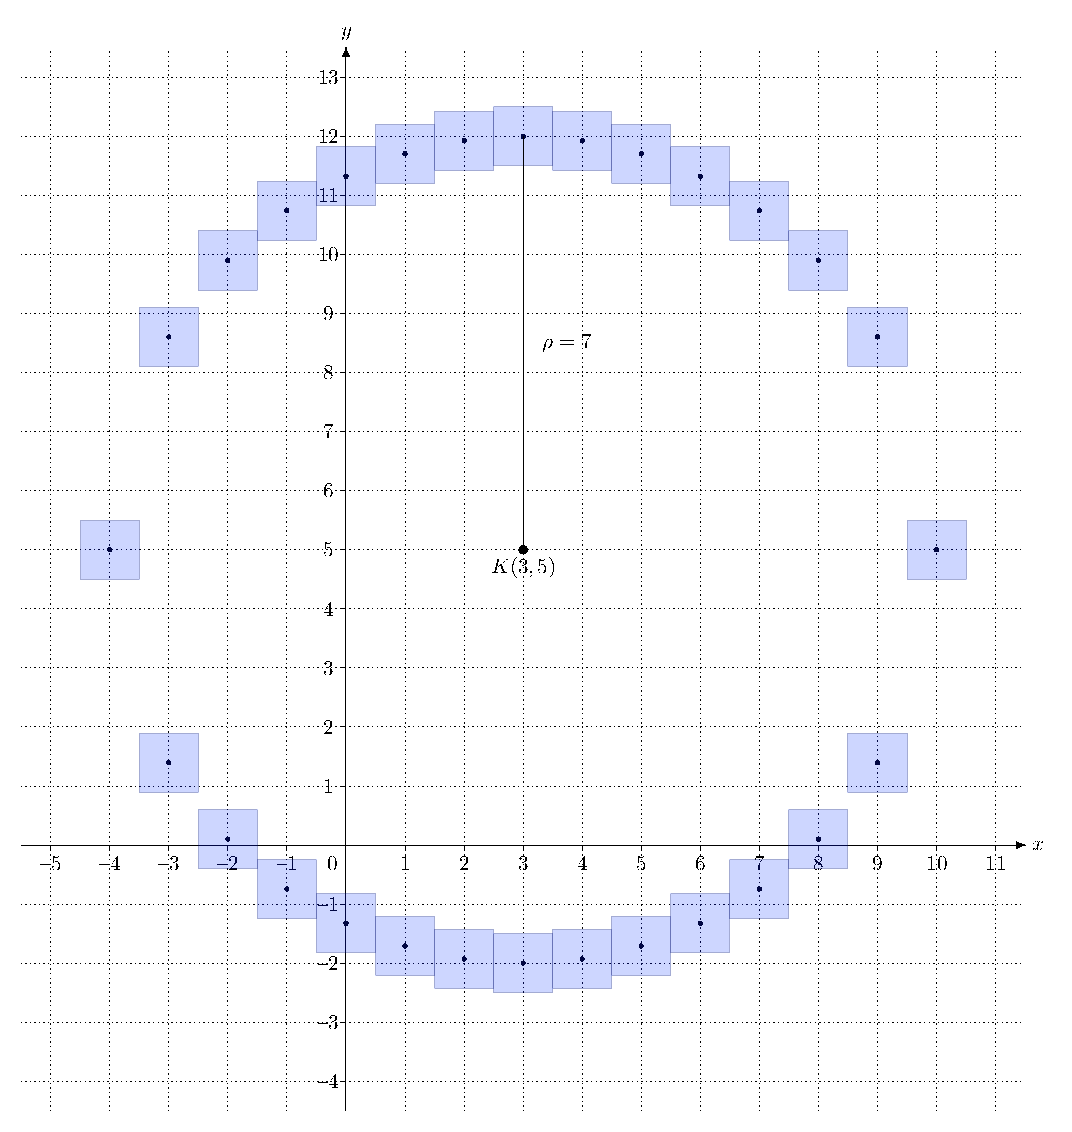
\includegraphics[scale=0.6]{Chapter1/Circle/plot-circle.pdf}
  \end{center}
  \caption{Σχεδιασμός κύκλου κέντρου $K(3,5)$ και ακτίνας $r=7$ μέσω αλγεβρικής εξίσωσης}
\end{figure}

Ο αλγόριθμος αυτός μπορεί να βελτιωθεί αν χρησιμοποιήσουμε τις παραμετρικές εξισώσεις για τις συντεταγμένες του κύκλου.
\begin{equation*}
	  \left.\begin{aligned}
	  x(t) &= x_c + r\cos{t}\\
	  y(t) &= y_c + r\sin{t}
	\end{aligned}\right. \, , \, t \in [0, 2\pi]
\end{equation*}

\begin{lstlisting}[caption={Αλγόριθμος Σχεδιασμού Κύκλου μέσω παραμετρικής εξίσωσης}]
function circlePlot(xc, yc, r, iterations)
    # xc, yc are the coordinates of the circle's center
    # r is the radius of the circle

    theta_values = range(0, 2π, length=iterations)  # Even partition of [0, 2π]

    x_points = Float64[]  # To store x(t)
    y_points = Float64[]  # To store y(t)

    for t in theta_values
        x = xc + r * cos(t)
        y = yc + r * sin(t)
        push!(x_points, x)
        push!(y_points, y)
    end

    return x_points, y_points  # Return arrays of x and y coordinates
end
\end{lstlisting}



\begin{figure}[h!]
  \begin{center}
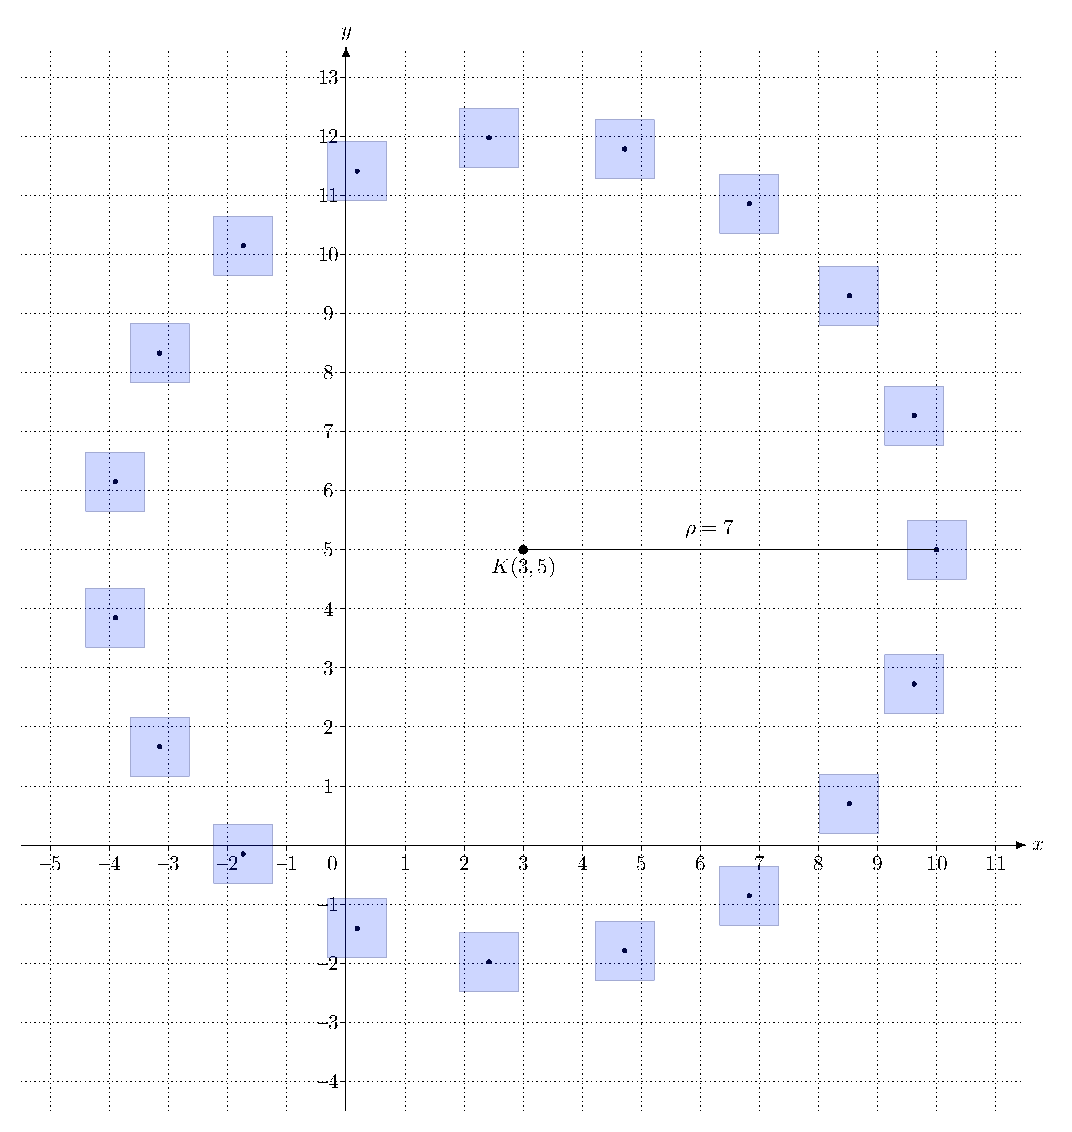
\includegraphics[scale=0.6]{Chapter1/Circle/circle-parametric.pdf}
  \end{center}
  \caption{Σχεδιασμός κύκλου κέντρου $K(3,5)$ και ακτίνας $r=7$ μέσω παραμετρικών εξισώσεων}
\end{figure}

Ενώ ο τρόπος αυτός σχεδιασμός κύκλου έχει πολύ καλά αποτελέσματα όσο αυξάνεται ο αριθμός επαναλήψεων (\texttt{iterations}), είναι αρκετά απαιτητικός καθώς απαιτεί για κάθε επανάληψη τις τιμές τριγωνομετρικών συναρτήσεων.
%%%%%%%%%%%%%%%%%%%%%%%%%%%%%%%%%%%%%%%%%%

\subsection{Σχεδιασμός κύκλου με τον Αλγόριθμο του Bresenham}

Ο κύκλος είναι ένα συμμετρικό σχήμα. Κάθε αλγόριθμος για τη σχεδίαση ενός κύκλου μπορεί να εκμεταλλευτεί αυτή τη συμμετρία για να σχεδιάσει $8$ σημεία υπολογίζοντας μόνο ένα. Αυτό αποτελεί τη λεγόμενη συμμετρία των $8$ δρόμων.

\begin{figure}[h!]
  \begin{center}
  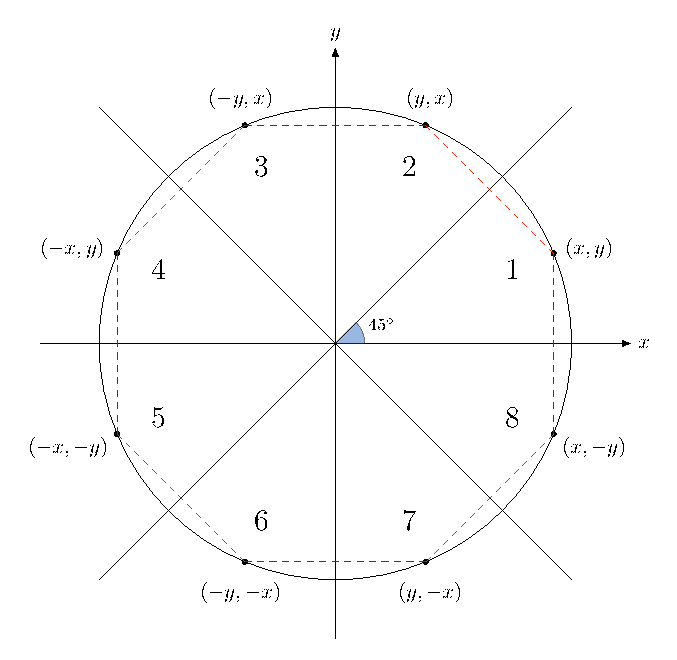
\includegraphics[scale=0.7]{Chapter1/Circle/8-street.pdf}
  \end{center}
  \caption{Συμμετρία των 8 δρόμων}
\end{figure}


Έστω ότι θέλουμε να σχεδιάσουμε το $2$ο οκτομόριο ενός κύκλου κέντρου $(0,0)$ και ακτίνας $\rho$. Εάν υπολογίσουμε όλα τα σημεία αυτού του οκταμορίου τα υπόλοιπα μπορούν να προσδιοριστούν χρησιμοποιώντας τη συμμετρία των $8$ δρόμων.


\subsection{Καθορισμός της μεταβλητής απόφασης}


Εάν φωτιστεί το pixel $(x_i, y_i)$ στο $2$ο οκταμόριο. Τα επόμενα δυνατά προς φωτισμό pixel θα είναι τα $(x_i + 1, y_i)$ ή $(x_i + 1, y_i - 1)$. 

\begin{figure}[hbt]
  \begin{center}
	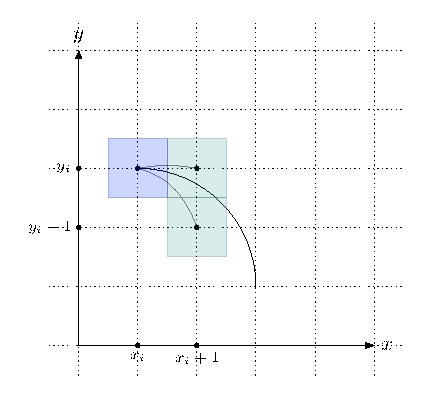
\includegraphics[scale=1]{Chapter1/Circle/circle-next-step.pdf}
  \end{center}
  \caption{Δίλημμα επιλογής επόμενου προς χρωματισμό pixel κατά τον σχεδιασμό του κύκλου σύμφωνα με τον αλγόριθμο του Bresenham}
\end{figure}

Θα πρέπει να καθορίσουμε μια μεταβλητή απόφασης ανάλογα με την οποία να επιλέγουμε εάν η συντεταγμένη $y$ θα παραμείνει ίδια ή θα ελαττωθεί, δεδομένου ότι η συντεταγμένη $x$ σταθερά θα αυξάνεται κατά $1$. 

Έστω ότι συντεταγμένη $x_{i+1}$ αντιστοιχεί σε κάποιο $y$ ανάμεσα στις τιμές $y_i$ και $y_i-1$. Είναι γνωστό ότι το σημείο $(x_i +1, y)$ θα ανήκει στον κύκλο, επομένως  το $y$ ικανοποιεί τη σχέση:
\[
	y^2 = r^2 - x_{i+1}^2.
\]

Ορίζουμε τις ακόλουθες διαφορές $d_1$ και $d_2$
\begin{align*}
	d_1 &= y_i^2 - y^2 = y_i^2 - r^2 + x_{i+1}^2 \\
	d_2 &= y^2 - \color{red}{(y_i-1)^2} = r^2 - x_{i+1}^2 - (y_i - 1)^2
\end{align*}

Εάν θέσουμε $e_i = d_1 - d_2$ τότε αυτή αποτελεί μεταβλητή απόφασης ανάλογα με το πρόσημο της οποίας μπορούμε να επιλέξουμε το επόμενο προς φωτισμό σημείο. Παρατηρούμε ότι


\begin{table}[htb]
\centering
	\begin{tabular}{@{}c|c@{}}
    \toprule
    $e_i$   & Επόμενο προς φωτισμό pixel \\ \midrule
    $<0$    & $(x_i + 1, y_i)$           \\
    $\geq 0$ & $(x_i + 1, y_i - 1)$      \\ \bottomrule
    \end{tabular}
\end{table}

Ο Bresenham απέδειξε ότι μία ικανοποιητική μεταβλητή απόφασης για την επιλογή του κατάλληλου pixel στο βήμα $i$ είναι η $e_i = d_1 - d_2$.


\subsection{Δημιουργία αναδρομικού τύπου}

Η μεταβλητή απόφασης $e_i$ μπορεί να υπολογισθεί ως εξής: 

\begin{align*}
	e_i &= d_1 - d_2 = 
		  y_i^2 - r^2 + (x_i +1)^2 - r^2 + (x_i +1)^2 + (y_i-1)^2 =  \\ 
		&=  2(x_i +1)^2 + y_i^2 + (y_i -1)^2 -2r^2	
\end{align*}
%
Επομένως:
%
\begin{align*}
	e_{i+1} &= 2(x_{i+1} + 1)^2 + y_{i+1}^2 + (y_{i+1}-1)^2 - 2r^2 = \\
			 &= 2(x_i +2)^2 + y_{i+1}^2 + (y_{i+1} -1)^2 - 2r^2 = \\
			 &= 2x_i^2 + 8x_i + 8 + y_{i+1}^2 + y_{i+1}^2 -2y_{i+1} + 1 -2r^2 = \\
			 &= (2x_i^2 + 4x_i +2) + 4x_i + 6 + 2y_{i+1}^2 -2y_{i+1} +1-r^2 = \\
			 &= 2(x_i +1)^2 + 4x_i + 6 + 2y_{i+1}^2 - 2y_{i+1} + 1 -2r^2 = \\
			 &= e_i - y_i^2 - y_i^2 + 2y_i -1 + 4x_i + 6 + 2y_{i+1}^2 -2y_{i+1} + 1 = \\
			 &=  e_i + 4x_i + 6 + 2(y_{i+1}^2 - y_i^2) -2(y_{i+1} - y_i)
\end{align*}
%
Άρα:
%
\begin{equation}
	e_{i+1} = e_i + 4x_i + 6 + 2(y_{i+1}^2 - y_i^2) -2(y_{i+1}-y_i)
	\label{eq:2}
\end{equation}


Επειδή στη σχεδίαση του $2$ου οκταμορίου ξεκινάμε από το $(x_1, y_1) = (0,r)$, η αρχική μεταβλητή απόφασης $e_1$ είναι:
%
\begin{align*}
	e_1 = 2+r^2 + (r-1)^2 - 2r^2 = 
		2+r^2 + r^2 -2r+1-2r^2 = 
		3-2r.
\end{align*}

Επειδή στο δεύτερο οκταμόριο η τιμή του $y_{i+1}$ είναι $y_i$ ή $y_i -1$ (μεγαλύτερη ταχύτητα στη $x$ κατεύθυνση) μπορούμε να υπολογίσουμε το $e_{i+1}$ με βάση το πρόσημο του $e_i$ ως εξής.

\begin{itemize}
  \item $e_i < 0 \Rightarrow y_{i+1} = y_i$. Τότε η \eqref{eq:2} γίνεται:
  \[
	   e_{i+1} = e_i + 4(x_i +1) + 2 \Rightarrow e_{i+1} = e_i + 4(x_i + 1) + 2
   \]
   \item $e_i \geq 0 \Rightarrow y_{i+1} = y_i - 1$. Τότε η \eqref{eq:2} γίνεται:
   \begin{align*}
   	e_{i+1} &= e_i + 4x_i  + 6 + 2( (y_i -1)^2 - y_i^2 ) - 2(y_i -1 -y_i) =  \\
   			&= e_i + 4x_i + 6 + 2(y_i^2 -2y_i + 1 -y_i^2) + 2 = \\ 
 			&= e_i + 4(x_i + 1) + 2 -4(y_i -1)
   \end{align*}
   
\end{itemize}

Ανάλογα λοιπόν με το πρόσημο της μεταβλητής $e_i$ έχουμε:

\begin{table}[htb]
\centering
    \begin{tabular}{@{}c|c@{}}
        \toprule
        $e_i$    & $e_{i+1}$                         \\ \midrule
        $<0$     & $e_i + 4(x_i +1) +2$              \\
        $\geq 0$ & $e_i + 4(x_i +1) +2 - 4(y_i - 1)$ \\ \bottomrule
    \end{tabular}
\end{table}



\subsection{Αλγόριθμος Bresenham για κύκλο}

Για να σχεδιάσουμε κάποιο κύκλο με διαφορετικό κέντρο, αρκεί να παρατηρήσουμε αν εφαρμόσουμε μετασχηματισμό μεταφοράς, ότι ένα σημείο της περιφέρειας ενός τέτοιου κύκλου μπορεί να σχεδιαστεί αν μεταφέρουμε τον κύκλο με κέντρο το $(0,0)$ κατά διάνυσμα με συντεταγμένες το κέντρο του κύκλου. Έτσι προκύπτει ο ακόλουθος αλγόριθμος υλοποιημένος σε Julia.

Τα παραπάνω μας οδηγούν στον παρακάτω αλγόριθμο χρησιμοποιώντας και την συμμετρία των $8$ δρόμων.

\begin{lstlisting}[caption={Bresenham Circle Algorithm}]
function bresenhamCircle(r)
	# (xc, yc) are the coordinates of the circle's centre
	# r is the radius of the circle
	x = 0 
	y = r
	error = 3 - 2 * r
	
	while x <= y
		plot(x, y)
		 
		plot(x+xc, y+yc, 0)
		plot(x+xc, -y+yc, 0) 
		plot(-x+xc, y+yc, 0) 
		plot(-x+xc, -y+yc, 0) 
		plot(y+xc, x+yc, 0) 
		plot(-y+xc, x+yc, 0)
		plot(y+xc, -x+yc, 0) 
		plot(-y+xc, -x+yc, 0) 
		x = x + 1
		if error > 0
			y = y - 1
			error = error - 4*y
		end
		error = error + 4*x +2
	end
end
\end{lstlisting}



\begin{figure}[hbt]
  \begin{center}
	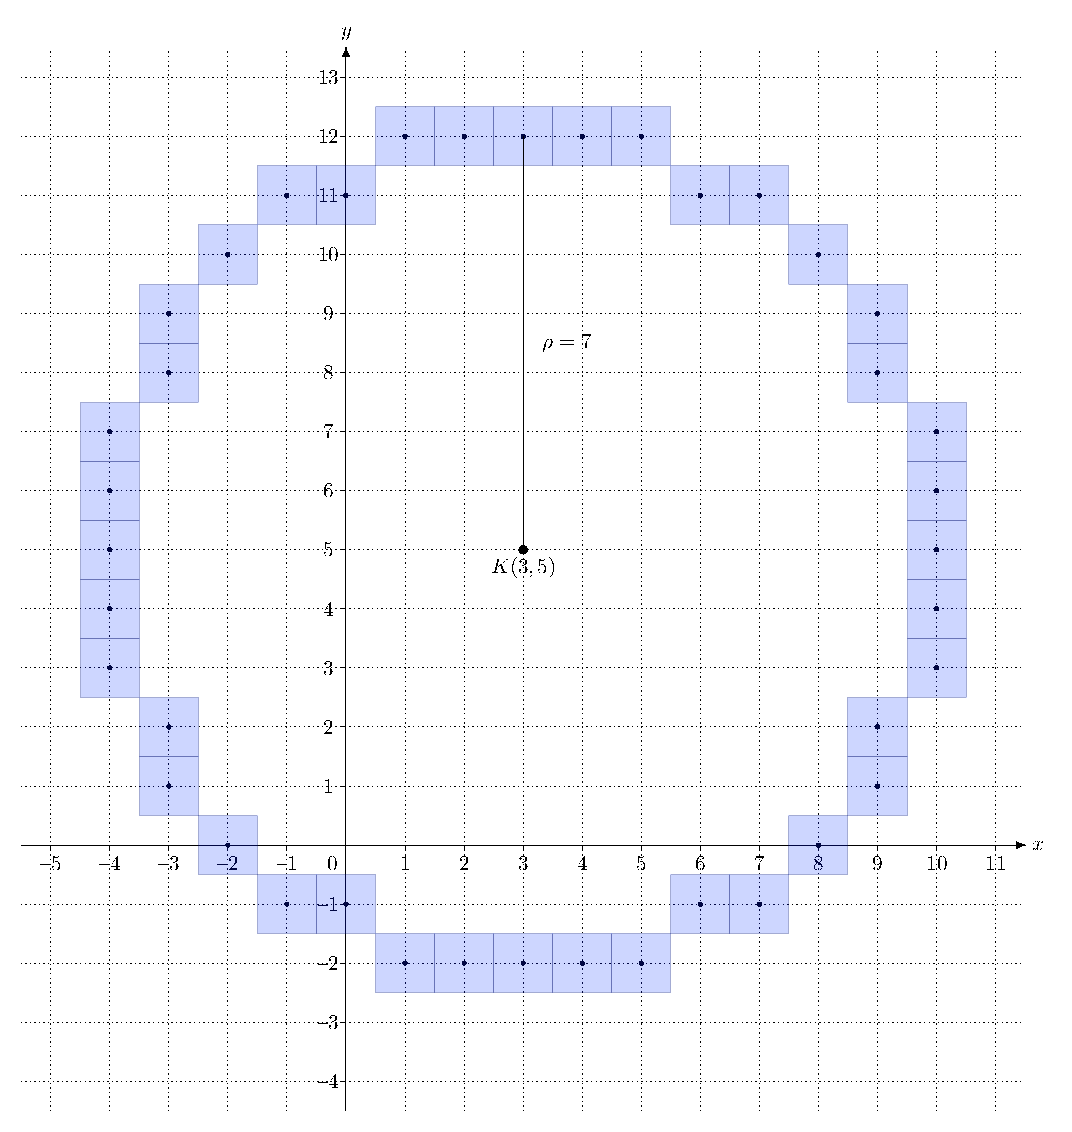
\includegraphics[scale=0.6]{Chapter1/Circle/bresenham-circle-example.pdf}
  \end{center}
  \caption{Παράδειγμα κύκλου με κέντρο $K(3,5)$ και ακτίνα $\rho = 7$}
\end{figure}


\subsection{Υπολογιστική Πολυπλοκότητα}

Στο $2$ο οκταμόριο ισχύει : $0 \leq r\cos{\ang{45}}, r \sin{\ang{45}} \leq  y \leq  r$. Στην $x$ κατεύθυνση γίνονται $r \cos{\ang{45}}$ βήματα που αντιστοιχούν σε $ r(1 - \sin{\ang{45}})$ βήματα στην $y$ κατεύθυνση. Συνολικά σχεδιάζονται (υπολογίζονται) $r \cos{\ang{45}}$ σημεία.


\begin{figure}[hbt]
  \begin{center}
	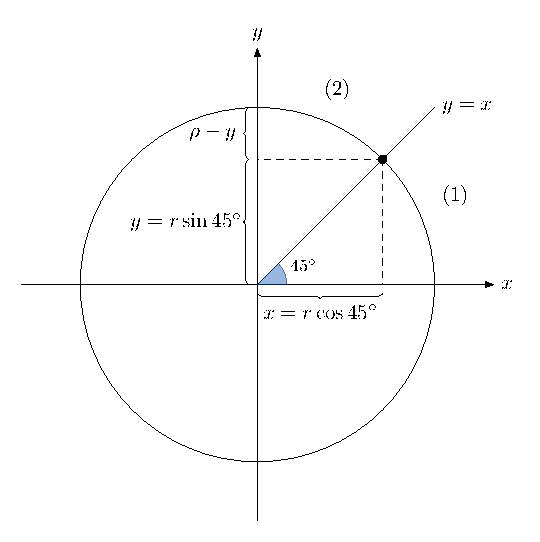
\includegraphics[scale=1]{Chapter1/Circle/circle-complexity.pdf}
  \end{center}
  \caption{Παράδειγμα κύκλου με κέντρο $K(3,5)$ και ακτίνα $\rho = 7$}
\end{figure}





Μέσος όρος βημάτων:
\[
	\left( \cfrac{r\cfrac{\sqrt{2}}{2} + r - r\cfrac{\sqrt{2}}{2} }{r\cfrac{\sqrt{2}}{2}} \right) = \sqrt{2}
\]


Η εντολή \texttt{error = error + 4x + 2} περιλαμβάνει $2$ προσθέσεις, $1$ shift πράξη (πολλαπλασιασμός με $2$). Τελικά κατά μέσο όρο έχουμε $4\sqrt{2}$ προσθέσεις, $2$ shift και $\sqrt{2}$ increments (αυξήσεις) ανά σχεδίαση σημείου του κύκλου.
Αν οι πράξεις εντός του \texttt{while} απαιτούν $1$ κύκλο hardware, τότε για το $2$ο οκταμόριο απαιτούνται $\sqrt{2}$ κύκλοι ανά σημείο. Για ολόκληρο κύκλο $(7+ 2) /8$ κύκλοι ανά σημείο, δηλαδή $1.05$ κύκλοι ανά σημείο.
\begin{remark}
Τα συνολικά σημεία που σχεδιάζονται στον κύκλο είναι $8r \cos{\ang{45}} = 4r \sqrt{2}$. Συγκρινόμενα με την περίμετρο $2 \pi\rho$ είναι $10\%$ λιγότερα. 
\end{remark}